%https://www.integral-domain.org/lwilliams/Resources/TikzImg/hexpaper.tex
\documentclass[tikz]{standalone}

\begin{document} 
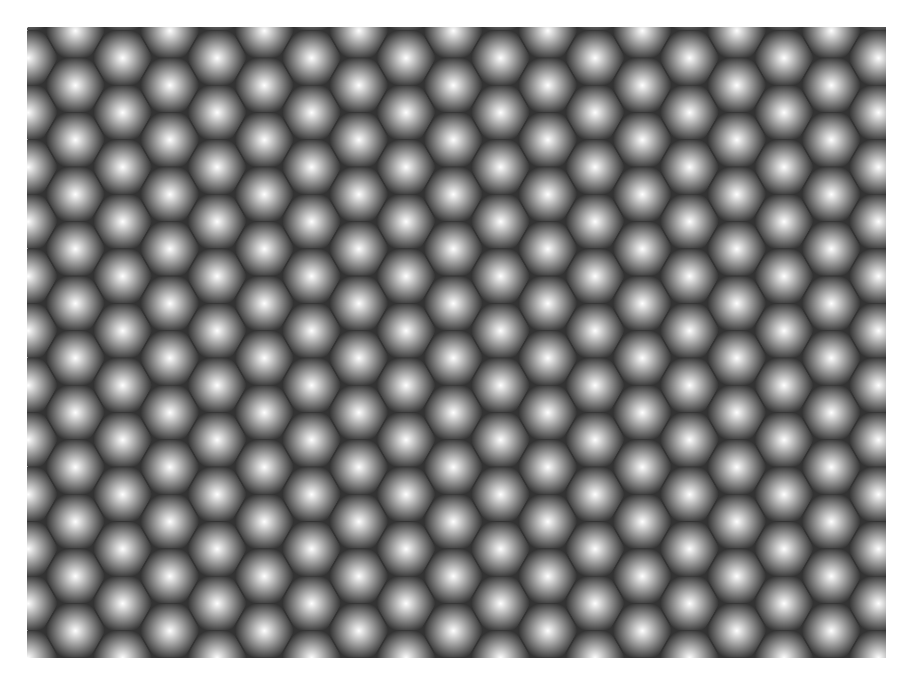
\begin{tikzpicture}

% paper size:
\pgfmathsetmacro\pwidth{10.9};
\pgfmathsetmacro\pheight{8};
% hexagon radius:
\pgfmathsetmacro\R{0.4};
 
\clip(0,0) rectangle (\pwidth,\pheight); 

\pgfmathsetmacro\ncols{\pwidth/(\R*1.5)}
\pgfmathsetmacro\nrows{\pheight/(\R*1.6)}

\newcommand{\thisshape}[3]{
  \draw[thin,shade,inner color=#1,outer color=#2, draw=#3,shading angle=45] (300:\R)--(0:\R)--(60:\R)--(120:\R)--(180:\R)--(240:\R)
}
\foreach \col in {0,2,4,...,\ncols}{
  \foreach \row in {0,1,2,...,\nrows} {
    \begin{scope}[xshift=1.5*\R*\col cm,yshift=2*0.866*\R*\row cm]
       \thisshape{white}{black!80}{black!80};
       %\thisshape{black!220!white}{white}{white};
    \end{scope}
  }
}
\foreach \col in {1,3,5,...,\ncols}{
  \foreach \row in {0,1,2,3,...,\nrows} {
    \begin{scope}[xshift=1.5*\R*\col cm,yshift=2*0.866*\R*\row cm -0.866*\R cm]
      \thisshape{white}{black!80}{black!80};
      %\thisshape{black!220!white}{white}{white};
    \end{scope}
  }
}

\end{tikzpicture} 
\end{document}